


\section{Compensating pairs of paths}
\label{Sec.comp}

In this section, we explore the key factor for the loss of accuracy in value 
abstraction methodologies. To this end, we first introduce the novel notion of compensating paths:

\begin{definition}
A pair $(\pi,\pi')$ of paths is {\em compensating} if:
\begin{itemize}
	\item they have the same starting node $a$ (called {\em source} state) and ending node $b$ (called {\em target} state of $(\pi,\pi')$),
	\item they are disjoints (the only common nodes are the source and the target),
	\item the weights satisfy $weight(\pi') < 0 < weight(\pi)$.
\end{itemize}	
We call a path $\pi$ {\em compensating} if there exists a path $\pi'$ such that either $(\pi,\pi')$ or $(\pi',\pi)$ is compensating.
\end{definition}

\begin{example}
	For instance, on Fig.~\ref{fig1}, the paths $\pi= n_2 n_3 n_5$ has weight $1$, while the
	path $\pi'= n_2 n_4 n_5$ has weight $-2$, hence $(\pi,\pi')$ is a compensating pair of paths.
	\end{example}


The phenomenon of compensating pairs of paths significantly impacts the precision of the target state due to the overabstraction of values. For instance, consider a scenario where $x_5 \leq 4$ is attainable when $x_1=1$ and $x_2=-1$, leading to $\val_{(1,-1)}(n_5)=4$. However, the Box methodology estimates an upper limit of $6$. Although DeepPoly partially rectifies the dependency on $x_2$, it achieves only partial negation of the $x_2$ value owing to the excessive abstraction characteristic of ReLU. This results in an overestimated upper bound of $x_5 \leq 5$ through a contribution of $\frac{-x_2+3}{2} \leq 2$, as opposed to the exact calculation of $-x_2 \leq 1$, culminating in a precise upper bound of $x_5 \leq 4$.

In an intuitive sense, the target state accrues weight from the source state via different paths connecting the source to the target. When these connecting paths possess weights of contrasting signs, a certain degree of cancellation occurs, with the extent of cancellation being up to $min(|weight(\pi')|,|weight(\pi')|)$. This mechanism also serves to mitigate error propagation in a manner similar to how $0 = |1+(-1)| \leq |1|+|-1| = 2$ in imprecise analyses. However, the ReLU functions can constrain the level of compensation due to their clipping effect. For instance, if the inputs $x_1, x_2$ are confined within the range $[-1,-0]$, then $\hat{x}_3$ will consistently be 0 for any input $\vx=(x_1,x_2)$ within the domain $[-1,-0] \times [-1,-0]$, thereby preventing $weight(\pi')$ from effectively counterbalancing $weight(\pi')$.




\iffalse
\vspace*{2ex}

\begin{figure}
	\centering
	\begin{tikzpicture}
		
		\node[circle, draw= purple, thick, minimum width = 20,
		minimum height = 20] (input1) {$a$};
		
		
		% Hidden layers
		\node[circle, draw= blue, thick, minimum width = 20,
		minimum height = 20] (hidden1) at ($(input1) + (2,1)$) {$b$};
		\node[circle, draw= blue, thick] (hidden2) at ($(input1) + (2,-1)$) {$b'$};
		
		\node[circle, draw= blue, thick, minimum width = 20,
		minimum height = 20] (hidden3) at ($(input1) + (4,1)$){$c$};
		\node[circle, draw= blue, thick] (hidden4) at ($(input1) + (4,-1)$) {$c'$};
		
		% Output layer
		\node[circle, draw= blue, thick, minimum width = 20,
		minimum height = 20] (output) at ($(input1) + (6,0)$){$d$};
		
		% Connections
		\draw[->,thick,draw= red] (input1) -- (hidden1) node[midway, below] {$1$};
		\draw[->,thick,draw= green] (input1) -- (hidden2)node[midway, below] {$-1$};
		
		\draw[->,thick,draw= red] (hidden1) -- (hidden3) node[midway, below] {$\ReLU$};
		\draw[->,thick,draw= green] (hidden2) -- (hidden4) node[midway, below] {$\ReLU$};
		
		\draw[->,thick,draw= red] (hidden3) -- (output)node[midway, below] {$1$};
		\draw[->,thick,draw= green] (hidden4) -- (output)node[midway, below] {$1$};
	\end{tikzpicture}
\end{figure}

\vspace*{2ex}

In this figure, $a$ is the input neuron; $bc,b'c'$ are nodes in the hidden layer, ($b,b'$ are pre-activation and $c,c'$ are post activation); and $d$ is the unique output neuron. The numbers next to the arrows are the weights. So, $W_{ba}=1$ and $W_{b'a}=-1$, $W_{dc}=W_{dc'}=1$. The pair of these two paths, $a$ to $bc$ to $d$, and $a$ to $b'c'$ to $d$, is a so called \emph{Compensating Pair}. Because its shape looks like a diamond, it is also called a Diamond. The characteristic is that, the products of all weights in the paths, have two different signs: along $bc$, the product is (strictly) positive, while along $b'c'$, the product is (strictly) negative. 

The existence of compensating pairs is key reason why simple approximation like LP or Interval Arithmetic cannot get the exact upper and lower bounds. If both pairs are negative or positive, LP or even Interval Arithmetic will get the exact values of lower and upper bounds.


To explain why, suppose we have another input node $a'$, such that both $a$ and $a'$ has an input interval $[0,1]$, but the weight from $a'$ to $b$ or $b'$ are both $1$. Then both $b$ will have an interval $[0,2]$ and $b'$ will have an interval $[-1,1]$. More importantly, in LP formulation, $c$ will be $b$ but $c'$ will be $0.5(b')+0.5$. The upper bound of $d$ will be $c+c'$, and hence $b+0.5(b')+0.5$, and hence $a+a'+0.5a'-0.5a'+0.5=0.5a+1.5a'+0.5$. And this will leads to a upper bound $2.5$ but this is not exact.

\vspace*{2ex}
\begin{tikzpicture}
	\node[circle, draw= purple, thick, minimum width = 20,
	minimum height = 20] (input1) {$a$};
	
	\node[circle, draw= purple, thick, minimum width = 20,
	minimum height = 20] (input2) at ($(input1) + (0,-2)$) {$a'$};
	
	
	% Hidden layers
	\node[circle, draw= blue, thick, minimum width = 20,
	minimum height = 20] (hidden1) at ($(input1) + (2,0)$) {$b$};
	\node[circle, draw= blue, thick] (hidden2) at ($(input1) + (2,-2)$) {$b'$};
	
	\node[circle, draw= blue, thick, minimum width = 20,
	minimum height = 20] (hidden3) at ($(input1) + (4,0)$){$c$};
	\node[circle, draw= blue, thick] (hidden4) at ($(input1) + (4,-2)$) {$c'$};
	
	% Output layer
	\node[circle, draw= blue, thick, minimum width = 20,
	minimum height = 20] (output) at ($(input1) + (6,-1)$){$d$};
	
	% Connections
	\draw[->,thick,draw= red] (input1) -- (hidden1);
	\draw[->,thick,draw= green] (input1) -- (hidden2);
	
	\draw[->,thick,draw= red] (input2) -- (hidden1) node[midway, below] {$1$};
	\draw[->,thick,draw= red] (input2) -- (hidden2)node[midway, below] {$1$};
	
	\draw[->,thick,draw= red] (hidden1) -- (hidden3) node[midway, below] {$\ReLU$};
	\draw[->,thick,draw= green] (hidden2) -- (hidden4) node[midway, below] {$\ReLU$};
	
	\draw[->,thick,draw= red] (hidden3) -- (output)node[midway, below] {$1$};
	\draw[->,thick,draw= green] (hidden4) -- (output)node[midway, below] {$1$};
\end{tikzpicture}
\vspace*{2ex}

The general formal definition of compensating pair is as follows:

\begin{definition} In a full-connected network with $\ReLU$ as activation function:
	
	1. A path is a sequence of nodes $\langle a,b,c,d,e,\cdots\rangle$ of nodes that goes consecutively through each layer. We call the first node source node and the last node target node.  
	
	2. The \emph{Value} of a path is the product of of weights along the path (with sign): for a path $\langle a,b,c,d,e,\cdots\rangle$, its values is $$V = W_{ab}\cdot W_{bc}\cdot W_{cd}\cdot W_{ed}\cdot \cdots$$
	
	3. A \emph{Compensating Pair} is a pair of paths with the same source node and target node, such that the two paths have no common node, and the values of two paths have opposite signs (one is strictly positive and another is strictly negative).
	
	We also use \emph{Diamond} to call a compensating pair in the network.
\end{definition}

The following theorem shows the role of compensating pairs in the computation:

\fi

\begin{table}[b!]
	\centering
	\begin{tabular}{|c|c|c|c|}
		\hline
		\text{Source/Target Layers}  &  \text{Natural DNN} & \text{Robust DNN} & \text{Ratio Natural vs Robust} \\ \hline \hline
		0 / 2 & 0.0304 & 0.00220  & 13.8x\\ \hline
		1 / 3  & 0.0313 & 0.00875 & 3.58x \\ \hline
		2 / 4  &  0.0267 & 0.00785 & 3.40x \\ \hline
		3 / 5  &  0.0253 & 0.00804  & 3.18x \\ \hline
	\end{tabular}
	\caption{Comparison of the average compensation strength over all the pairs of nodes of layer source/target between a DNN naturally-trained and a DNN robustly-trained using DiffAI \cite{DiffAI} with the same architecture and training set.}
	\label{tab:compensation}
\end{table}


The discussion so far shows  that compensation is one of the possible factors contributing to inaccuracy. We now establish that it is the sole cause of inaccuracy:
if a DNN lacks any compensating path, then any methodology that is at least as accurate as the Box abstraction, such as LP and $\overline{\mbox{DeepPoly}}$ (but not DeepPoly), will precisely determine the exact upper and lower bounds for every node. This assertion is formalized in the following theorem:

\begin{theorem}
	\label{th1}
	Consider any node $n$ within a DNN devoid of any compensating path. Let $[\alpha,\beta]$ represent the bounds computed by the Box abstraction for node $n$. Then, for every $\gamma$ within the interval $[\alpha,\beta]$, there exists an input $\vx$ such that $\val_{\vx}(n) = \gamma$.
\end{theorem}

The sketch of proof can be found in Section \ref{sec.proofs}. 

This theorem underscores the significant role of compensating paths in the accuracy of bound estimation within DNNs, affirming that their absence guarantees the precision of computed bounds. Practically speaking, encountering a network entirely devoid of compensating paths is highly improbable, rendering this more a theoretical observation, highlighting that compensation is a key driver of inaccuracy.




%It is worth remarking that  Theorem~\ref{th1} does not directly apply to standard DeepPoly since DeepPoly does not inherently refine the Box abstraction.  Furthermore, it is unclear whether  Theorem~\ref{th1} applies to PRIMA or $\beta$-CROWN as these techniques refine DeepPoly.  Nevertheless, this limitation could potentially be addressed by integrating $\overline{\text{DeepPoly}}$.

An intriguing application of this result lies in elucidating why certain DNNs are inherently more amenable to verification compared to others. This distinction is notably evident between DNNs adversarially trained for robustness and those trained naturally, utilizing the same architecture \cite{deeppoly,prima,crown}. Notably, the presence of compensating pairs is an intrinsic structural attribute of the learned DNN, contrasting with more semantic aspects like the number of unstable ReLUs, which are significantly influenced by the specific image and algorithm employed. To illustrate this point, we consider two networks, each comprising 5 hidden layers with 100 nodes, sourced from the ERAN GitHub repository. One is naturally trained ($6\times100$), and the other is trained using DiffAI ($5\times100$). In Table \ref{tab:compensation}, we present the average compensation strength, computed as the mean of $max_{\pi,\pi'} min(|weight(\pi')|,|weight(\pi')|)$ across all source/target states within specified layers. The findings reveal that the average compensation strength is considerably lower in the Robust DNN compared to the natural DNN. Correspondingly, the Robust DNN is substantially easier to verify than its natural counterpart, as evidenced by the enhanced accuracy and image verification rate of DeepPoly.


\subsection{MILP$_{X_n}$}



While Theorem \ref{th1} is interesting to understand that compensation is a key notion for accurate verification of DNNs, it cannot be used directly to analyze DNNs with compensations, which are actually those that are most interesting to tackle.
Intuitively, when there are compensating paths, it seems necessary to consider exactly the (unstable) ReLU nodes that are seen along these paths. 
%Consider a neuron $n$ in layer $k$ for which we want to have accurate bounds 
%$[\alpha,\beta]$.

Consider a neuron $n$ in layer $k$, for which we aim to establish accurate bounds $[\alpha,\beta]$. Define $X_n$ as the set of neurons $x$ in layers up to $k-1$, where each $x$ is part of a compensating path targeting neuron $n$, but not as the source or the target node of the path. Let $Y_n$ represents the set of all other neurons in the first $k-1$ layers, essentially serving as the complement of $X_n$. We introduce MILP${X_n}$, a variant of the MILP encoding where all nodes in $Y_n$ are linearly relaxed, hence incorporating $|X_n|$ binary variables, each corresponding to a neuron in $X_n$. Additionally, this encoding encapsulates bounds for every neuron $n'$ in the initial $k-1$ layers, as computed inductively in previous steps. That is, we do not use explicitly in $X_n$ nodes on compensating paths with target neurons before $n$ ({\em indirectly} compensating paths), 
only those with target $n$ ({directly} compensating paths).
The contribution of these {\em indirectly} compensating paths are thus 
only taken into account indirectly via the bounds on previous neurons computed inductively,
and not as binary variables. We demonstrate now that the bounds $[\alpha,\beta]$ for neuron $n$, as computed by MILP${X_n}$, are accurate, thereby offering a more nuanced approach to DNN verification in scenarios involving compensating paths.
We will provide the proof under a fairly light well-connected hypothesis (H1), which only DNNs where all but very few weights are 0 does not satisfy.

(H1): for every 2 (not necessarily disjoint) paths $\rho_1,\rho_2$ with non-zero weight with the same source $m$ and the same target $n$ with at least 2 transitions, there exists another path $\rho_3$ from $m$ to $n$ (with non zero-weight) totally disjoint from $\rho_1$ and $\rho_2$ (except at the source and target). This hypothesis is used to remove corner cases which will not happen in actual DNNs, which all are well-connected.


\begin{theorem}
	\label{th2} 
	Assume the DNN satisfies the well-connected (H1) hypothesis.
	Let $n$ be any node of a DNN. Then for $[\alpha,\beta]$ the bounds computed by MILP$_{X_n}$ for neuron $n$, for all $\gamma \in [\alpha,\beta]$, there exists an input $\vy$ such that $\val_{\vy}(n)=\gamma$.
\end{theorem}

The sketch of proof of Theorem \ref{th2} can be found in Section \ref{sec.proofs2}.


\subsection{Sketch of Proof for Theorem \ref{th1}}
\label{sec.proofs}

First, notice that by continuity of all the functions used in the DNNs, it suffices to show both theorem for $\gamma=\alpha$ and $\gamma=\beta$.

%Intuitively, our first proof shows that if there are no compensation, then there are no correlations between nodes.
Consider a target neuron $z$.
In case there is no compensating path, we can assign a sign to each neuron $n$: 0
if all paths from $n$ to $z$ has weight 0, $+1$ if all paths have positive weights, and 
$-1$ if they have negative weights. 

Using the concept of sign, we introduce input vectors $\vx^{*}, \vx^{\sharp}$: 

\begin{definition}
We define the following two input vectors $\vx^{*}, \vx^{\sharp}$ in $\cal B$: 
	\begin{itemize}
		\item $\vx^{*}$ is the input vector defined in the following way:
		\begin {itemize}
		 \item $x^*_{a_i}=\max(a_i)$ if $S(a_i)\in \{0,1\}$, and
          \item $x^*_{a_i}=\min(a_i)$ otherwise, that is when $S(a_i)=-1$.
	\end{itemize}
		
		\item $\vx^{\sharp}$ is the input vector defined in the following way:
		\begin{itemize}
			\item $x^{\sharp}_{a_i}=\min(a_i)$ if $S(a_i)\in \{0,1\}$, and
			\item $x^{\sharp}_{a_i}=\max(a_i)$ otherwise, that is when $S(a_i)=-1$.
		\end{itemize}
	\end{itemize}
\end{definition}



We can then prove that $\vx^\star,\vx^\sharp$ maximize and minimize conjointly all the nodes in the DNN. Notice that it does {\em not} mean that there is no dependencies between nodes.
There can be correlations between nodes, just they do not affect the $\min$ and $\max$ bounds that can be reached in any node.

\begin{proposition}
	\label{prop.sign}
	${\vx^\star}$ maximizes the value of all positive neurons and minimizes the value of all negative neurons, and  
	${\vx^\sharp}$ minimizes the value of all positive neurons and maximizes the value of all negative neurons.
\end{proposition}

Hence $\val_{\vx^\star}(z)=\beta$ and $\val_{\vx^\sharp}(z)=\alpha$,
for $[\alpha, \beta]$ the bounds computed by the Box abstraction. We conclude Theorem \ref{th1} by invocking continuity.

\smallskip
The formal proof is in appendix A.


\subsection{Sketch of Proof for Theorem \ref{th2}}
\label{sec.proofs2}

\begin{figure}[h]
	\centering
	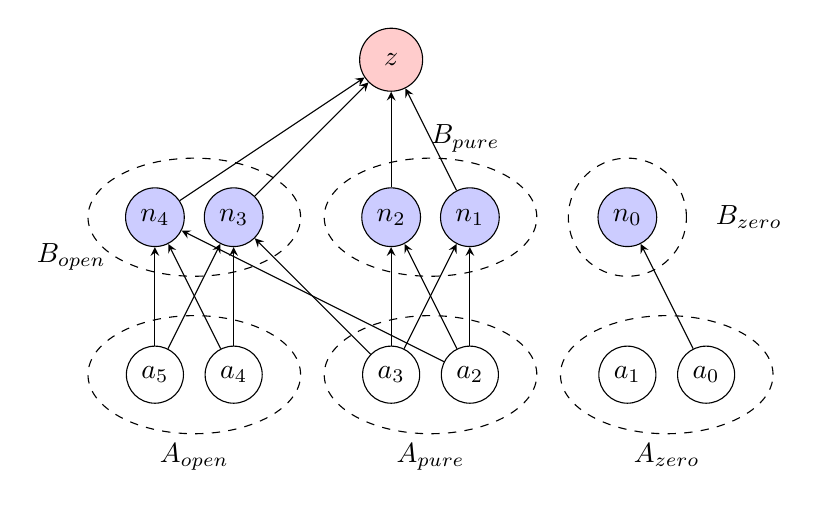
\begin{tikzpicture}[>=stealth, node distance=2cm]
		% Input nodes (two types)
		\node[circle, draw, minimum size=0.5cm] (input1) at (-1,0) {$a_0$};
		\node[circle, draw, minimum size=0.5cm] (input2) at (-2,0) {$a_1$};
		\node[circle, draw, minimum size=0.5cm] (input3) at (-4,0) {$a_2$};
		
		\node[circle, draw, minimum size=0.5cm] (input4) at (-5,0) {$a_3$};
		\node[circle, draw, minimum size=0.5cm] (input5) at (-7,0) {$a_4$};
		\node[circle, draw, minimum size=0.5cm] (input6) at (-8,0) {$a_5$};
	
		\draw[draw=black, dashed] (-1.5,0) ellipse (1.35 and 0.75);
		\node[below] at (-1.5,-0.75) {$A_{zero}$};
		
		\draw[draw=black, dashed] (-2,2) ellipse (0.75 and 0.75);
		\node[right] at (-1,2) {$B_{zero}$};
		
		% Hidden layer nodes
		
		\node[circle, draw, minimum size=0.5cm, fill=blue!20] (hidden1) at (-2,2) {$n_0$};
		
		\node[circle, draw, minimum size=0.5cm, fill=blue!20] (hidden2) at (-4,2) {$n_1$};
		\node[circle, draw, minimum size=0.5cm, fill=blue!20] (hidden3) at (-5,2) {$n_2$};
		
		\node[circle, draw, minimum size=0.5cm, fill=blue!20] (hidden4) at (-7,2) {$n_3$};
		\node[circle, draw, minimum size=0.5cm, fill=blue!20] (hidden5) at (-8,2) {$n_4$};
		
		
		
		\draw[draw=black, dashed] (-4.5,0) ellipse (1.35 and 0.75);
		\node[below] at (-4.5,-0.75) {$A_{pure}$};
		
		
		\draw[draw=black, dashed] (-7.5,0) ellipse (1.35 and 0.75);
		\node[below] at (-7.5,-0.75) {$A_{open}$};
		
		
		
		\draw[draw=black, dashed] (-4.5,2) ellipse (1.35 and 0.75);
		\node[left] at (-3.5,3) {$B_{pure}$};
		
		
		\draw[draw=black, dashed] (-7.5,2) ellipse (1.35 and 0.75);
		\node[left] at (-8.5,1.5) {$B_{open}$};
		
		
		
		% Output node
		\node[circle, draw, minimum size=0.8cm, fill=red!20] (output) at (-5,4) {$z$};
		
		
		% connections
		
		\draw[->] (input1) -- (hidden1);
		
		\draw[->] (input3) -- (hidden5);
		
		\draw[->] (input4) -- (hidden4);
		
		
%		% Connect input to hidden layer
		\foreach \i in {3,4} {
			\foreach \h in {3,2} {
				\draw[->] (input\i) -- (hidden\h);
			}
		}
		
		
		\foreach \i in {5,6} {
			\foreach \h in {4,5} {
				\draw[->] (input\i) -- (hidden\h);
			}
		}
%		
		% Connect hidden layer to output
		\foreach \h in {2,3,4,5} {
			\draw[->] (hidden\h) -- (output);
		}
		
%		% Input label
%		\node[left=0.5cm of input1] {Input Layer};
%		% Hidden label
%		\node[right=0.5cm of hidden2] {Hidden Layer};
%		% Output label
%		\node[right=0.5cm of output] {Output Layer};
	\end{tikzpicture}
	\caption{Simple Neural Network with Different Types of Input Nodes}
	\label{fig:neural_network_types_simplified}
\end{figure}

Concerning Theorem \ref{th2}, consider an output node $z$.
Let $[\alpha(z),\beta(z)]$ be the bound computed by $\MILP_{X_z}$.
%We will show the existence of $\vx^\sharp,\vx^\star$
%such that $\val_{\vx^\sharp}(z)=\alpha$ and $\val_{\vx^\star}(z)=\beta$,
%and we will get the proof of Theorem 2 by a continuity argument.
%For that, 
We partition the input neurons from layer $0$ into:
\begin{enumerate}
	\item $A_{zero}= \{a \mid \forall \text{ path $\rho$ from $a$ to } z, weight(\rho)=0\}$.
	\item $A_{pos}= \{a \mid \forall \text{ path $\rho$ from $a$ to } z, weight(\rho)\geq0\}$.
	\item  $A_{neg}= \{a \mid \forall \text{ path $\rho$ from $a$ to } z, weight(\rho)\leq0\}$.
	Let $A_{pure}=A_{pos} \cup A_{neg}$.
	\item $A_{open}$ is the set of remaining input neurons.
\end{enumerate}

We then partition the set of neurons in hidden layers: 
\begin{enumerate}
	\item $B_{zero}= \{n \mid \forall \text{ path $\rho$ from $n$ to } z, weight(\rho)=0\}$.
	\item $B_{open}$ is the set of neurones reachable with $>0$ weight from $A_{open}$ and such that there is at least one path to $z$ with non zero weight.
	\item $B_{pure}$ is the set of remaining neurons.
\end{enumerate}

We can show the following lemma:

\begin{lemma}
	$A_{pure} \cup B_{pure} $ forms a sub-network, denoted $D_I$. That is, 
	for $n \in B_{pure}$, for every path $\rho$ from $m$ to $n$
	either $m \in B_{pure}\cup I$ or $weight(\rho)=0$.
\end{lemma}

Hence, the value of any neuron $n$ in $A_{pure}$ or $B_{pure}$ is entirely determined by 
inputs in $A_{pure}$. 


We cannot define the Sign function on nodes from which a compensating path can be reached.
However, we can define the sign function for neurons in $A_{pure}$ and $B_{pure}$.
Further, the set of nodes on which the sign function is defined is suffix-closed:

\begin{lemma}
	Let $m,n$ be two nodes, such that $S$ is defined on $m$ and there is a path $\rho$ with non zero weight to a node $n$. Then $S$ is defined on $n$.
	Further, $S(n)= Sign(weight(\rho)) S(m)$.
\end{lemma}

We can apply Theorem \ref{th1} on the DNN made of nodes from $A_{pure}$ and $B_{pure}$, and obtain $\vx_{pure}^\star,\vx_{pure}^\sharp$ optimizing neurons in $A_{pure}$ or $B_{pure}$:

\begin{proposition}
For a node $b$ with $S(b)=1$:

$$\max(b)=\max_{\vx_{open}} \val_{\vx^{\star}_{pure},\vx_{open}}(b)$$
$$\min(b)=\min_{\vx_{open}} \val_{\vx^{\sharp}_{pure},\vx_{open}}(b)$$

and for $S(b)=-1$:
$$\max(b)=\max_{\vx_{open}} \val_{\vx^{\sharp}_{pure},\vx_{open}}(b)$$
$$\min(b)=\min_{\vx_{open}} \val_{\vx^{\star}_{pure},\vx_{open}}(b)$$
\end{proposition}

Consider the DNN $D'$ with input nodes $A_{open}$, where all the 
edges from $m \in A_{open} \cup B_{open}$ to $n$ are replaced by a bias 
(equals to the weight of the edge times the fix value $\val_{\boldsymbol{x}^\star_{open}}(m)$) for $n$ (we sum all these bias for a neuron $n$).
The values in $D'$ are the same as the values in $D$ for input $\vx^{\star}_{pure}$,
which suffices to reach the maximal value of $D$.
In $D'$, all the ReLU nodes are in $B_{open}$. 
Hence $\MILP_{B_{open}}$ computes the bounds accurately in $D'$.
It will compute the bound in the same way in $D$, hence we get $\beta=\max(z)$ for the target $z$. The formal proof is in appendix B.


\subsection{An efficient algorithm}


Leveraging Theorem \ref{th2}, it is theoretically feasible to procure accurate bounds by iteratively applying MILP$_{X}$ to each node, layer by layer. This sequential approach would yield precise bounds $[\alpha,\beta]$ for each node, which could then be utilized to calculate accurate bounds for subsequent layers. However, in a practical setting, this methodology may prove to be computationally inefficient. Typically, the set $X_n$ includes a substantial portion of the nodes from all preceding layers up to layer $k-1$ for a given node $n$ in layer $k$. Instead, an interesting trade off between speed and accuracy is to set a threshold on the strength of compensation. Paths falling below this threshold are deemed to not warrant an individual integer variable due to insufficient compensatory strength. We denote the resultant subset of nodes situated on paths with substantial compensation as $Z_n$. In practical applications, one might consider selecting the $K$ nodes that are involved in the most significant compensating paths to construct the set $Z_n$, with $K$ being a relatively small integer. This strategy effectively provides a trade-off between the algorithm's performance and the precision of the results. The detailed steps of this approach are outlined in the pseudo-code for \CMP presented in Algorithm \ref{algo1}.





\SetKwInput{KwInput}{Input}
\SetKwInput{KwOutput}{Output}

\begin{algorithm}[b!]
	\caption{CMP($K$)}
	\label{algo1}
	\KwInput{Bounds $[\alpha_n,\beta_n]$ for input nodes $n$ at layer $0$ (input neighbourhood)}
	
	\KwOutput{Bounds $[\alpha_n,\beta_n]$ for every node $n$}
	
	\For{layer $k=1 \cdots \ell$}{
		\For{neuron $n$ in layer $k$}{
			
			Compute $Z$ a set of $K$ nodes covering the compensating pairs of paths with target $n$
			with heaviest compensation
			
			Run MILP$_Z$ to obtain $[\alpha_n,\beta_n]$ from bounds of neurons in layers $< k$
		}
	}
\end{algorithm}	




CMP($K$) has a worst case complexity bounded by $O(N \MILP(N,K))$, 
where $N$ is the number of nodes of the DNN, 
and $\MILP(N,K)$ is the complexity of solving a MILP program with $K$ integer variables and $N$ linear variables.
We have $\MILP(N,K) \leq 2^K \LP(N)$ where $\LP(N)$ is the Polynomial time to solve a Linear Program with $N$ variables.

Notably, this complexity serves as an upper bound. For instance, solvers like Gurobi are quite adept and usually do not need to evaluate all $2^K$ ReLU configurations to deduce the bounds.
It's worth mentioning that the for loop iterating over neurons $n$ in layer $k$, as seen in line 2, can be executed in parallel. This is feasible because the computation only depends on bounds from preceding layers, not the current layer $k$. This parallelization results in a time complexity of $O(\sum_{i=1}^{\ell} \MILP(N_{i-1},K))$, where $\ell$ denotes the total number of layers and $N_i$ the count of neurons in layers $0, ..., i$.


Therefore, if $K$ is sufficiently small, Algorithm \ref{algo1} frequently invokes MILP (e.g., using Gurobi) with a manageable number of integer variables. This approach is expected to be efficient and yet remains fairly precise, as it can accurately compute (according to Theorem \ref{th2}) the most significant compensating path. The effectiveness of this strategy is further examined in the subsequent section.



\iffalse
\section{Verification Framework}



%Our experiments are carried by different version codes, and the global process has been changed. 

In this section, we will sketch the framework. 

\subsection{Structure}

\subsubsection*{Precomputation}

The open node chosen is the key part of the whole framework but costs a lot of time. So some computation (those do not rely on certain image and bounds) is moved to the precomputation part.

%The precomputation corresponds to the simplest case: source node fixed. We will compute and store a limited number of paths with highest (absolute) values before running any image. This does not rely on other parameters or results(bounds).
%
%Before build an MILP model and when choosing open nodes list,  the program will read the reference data combining with the data of bounds to continue the computation of open nodes. This will use much less time.



\subsubsection*{Process for one image} An image is the basic unit in whole process. The process of one image is simple: compute the concrete bounds of nodes layer by layer, use the bounds of previous layer to build MILP models of current layer. In one layer, nodes runs in parallel.

%Suppose we have reached a new layer $l_i$ and have upper and lower bounds of all nodes in previous layers. Then we will compute bounds of every node in $l_i$ in parallel using the data of bounds of previous nodes. The method is to build and optimize an MILP model.

%Some parameters may be changed during layers. Among all parameters, two groups are the most important: numbers of open nodes and local timeout parameters. Here, \emph{local} is opposite to \emph{global}. We have global timeout parameters for images and the whole running. Local timeout are used in one layer, one node, one model, or one loop in the optimization for a model.




%The open node chosen is the key part of the whole framework, and it will cost two much time without precomputation because we must do open node chosen for every node. 
%
%The precomputation corresponds to the simplest case: source node fixed. We will compute and store a limited number of paths with highest (absolute) values before running any image. This does not rely on other parameters or results(bounds).
%
%Before build an MILP model and when choosing open nodes list,  the program will read the reference data combining with the data of bounds to continue the computation of open nodes. This will use much less time.

\begin{algorithm}
	\caption{The Frame work}
	\KwData{Input Domain: $\mathcal{D}$}
	\KwResult{Bounds of all nodes: $\mathcal{B}$}
	
	Constant $\mathcal{R}$  \tcp*{Stored precomputation data}
	
	Constant $\boldsymbol{W}, \vb$ \tcp*{Weights and Bias of network}
	
	Constant Layers = $[0,1,2\cdots,L]$ \tcp*{lists of all layer}
	
	Constant NodesLayer = $[Nodes_0,Nodes_1,\cdots, Nodes_L]$ \tcp*{list of nodes in each layer}
	
	
	Initialize $\mathcal{B}$ = \{\} \tcp*{To store upper and lower bounds of all nodes}
	
	\For{$l$ in Layers}{
		\If{$l$ = 0}{
			
			$\mathcal{D}$, $\boldsymbol{W}, \vb$ $\rightarrow$ $\mathcal{B}_0$ = \{$x$: $(UB(x),LB(x))$,$\cdots$\} 
			\tcp*{Do linear transformation  from input to the first layer}
			
			Add \{$x$: $(UB(x),LB(x))$,$\cdots$\} to $\mathcal{B}$} 
		
		\Else{
			
			$l$, NodesLayer $\rightarrow$ $Nodes_l$ = $[x_0,x_1,\cdots]$
			
			\For{$x$ in $Nodes_l$}{
				$x$, $\mathcal{B}$, $\mathcal{R}$  $\rightarrow$ $\mathcal{O}$ \tcp*{To get the open node list $\mathcal{O}$}
				
				$\mathcal{B}$, $\boldsymbol{W}, \vb$, $\mathcal{O}$ $\rightarrow \mathcal{M}$  \tcp*{MILP model $\mathcal{M}$ for node $x$}
				
				\While{}{$\mathcal{M}$ $\rightarrow UB(x),LB(x)$ \tcp*{Optimization}}
				
				Add \{$x$: $(UB(x),LB(x))$\} to $\mathcal{B}$
				
				
			}
			
		}
		
		
	}
	
	\Return{$\mathcal{B}$}
	
\end{algorithm}

\subsubsection*{Process for one node}

The optimization of a model consists of loops. For each loop, the model will do optimization by a timeout and observe the result. If it gets improvement, then continue the loop until the optimize bounds or the longer timeout. Otherwise it will give up optimization and store the best bounds obtained so far.  



\subsubsection*{Global Process}

In the newest version, we do images by batches for 100 images each. For each batch, the running consists of three turns, very fast turn, fast turn and slow turn.

In the very fast turn, it will run DeepPoly for all images to get a preliminary bounds for all nodes and verify the easiest images. Images verified and images with false predication will be deleted from the image list.

Then sort all remain images by the size of uncertainty of DeepPoly from smaller to larger. The fast turn is to run the images from the smaller side to larger side until consecutive two images cannot be verified. All remain images and images tried but not verified will be put into the next list. And then run the list with parameters for slow turn.




\subsection{Parameters}

Parameters like open node parameter $O$ is important in the frame. Basically, all parameters will be reset after one image.

\subsubsection*{Global parameters}




\subsubsection*{Local parameters}

$O$ and timeout parameters for loops will change frequently during the loops of one node. These change will not reset until the end of one layer or one image.



\subsection{Other Setting}

In our experiments, we have not used PGD-attack to exclude some images. In principle, there is no obstacle to use PGD-attack.
\fi




